\documentclass[12pt,a4paper]{ltjsarticle}
\usepackage{luatexja}
\usepackage{luatexja-fontspec}
\usepackage{luatexja-ruby}
\usepackage{amsmath}
\usepackage{amsfonts}
\usepackage{amssymb}
\usepackage{amsthm}
\usepackage{graphicx}
\usepackage{fancyhdr}
\usepackage{geometry}
\usepackage{setspace}
\usepackage{array}
\usepackage{booktabs}
\usepackage{longtable}
\usepackage{url}
\usepackage{hyperref}
\usepackage{tikz}
\usepackage{pgfplots}
\pgfplotsset{compat=1.18}
\usepackage[font=normalsize]{caption} % キャプションのフォントサイズを標準に設定(エラー回避)

% URLの改行設定
\urlstyle{same}
\makeatletter
\def\url@samestyle{%
  \@ifundefined{selectfont}{\def\UrlFont{\sf}}{\def\UrlFont{\small\ttfamily}}}
\makeatother

% 日本語フォントの設定
\setmainjfont{Yu Mincho}[Scale=1]
\setsansjfont{Yu Gothic}[Scale=1]

\geometry{left=3cm,right=3cm,top=3cm,bottom=3cm}
\onehalfspacing

\title{\ruby{最速降下曲線}{さいそくこうかきょくせん}:単純な問いから美しい数学的真実への旅}
\author{}
\date{}

\begin{document}

\maketitle

\section{はじめに:究極のウォータースライダー問題}

もしあなたが、ある地点Aから、それより低い別の地点Bまで、最も速く滑り降りることができるウォータースライダーを設計するよう依頼されたとしたら、どのような形を思い描くでしょうか?地点Bは地点Aの真下ではなく、少し離れた場所にあるとします。

この問いに対して、私たちの直感はいくつかの答えを提案します。

まず考えられるのは、\textbf{候補1:直線}です。二点間の最短距離は直線であり、距離が最も短いのだから、時間も最も短くなるはずだ、と考えるのは非常に自然なことです。これは多くの人が最初に思いつく、論理的な推測でしょう。

次に、別の戦略が頭に浮かびます。\textbf{候補2:急降下}。最初に一気に加速すれば、後半で速さを稼げるのではないか、という考え方です。例えば、最初に垂直に落下して速度を最大にし、その後水平に進むような経路です。

しかし、ここにはこの問題の中心的な対立、つまり「\ruby{パズル}{謎}」が潜んでいます。直線経路は距離を最小化しますが、重力による加速が緩やかです。一方で、急降下経路は初期の加速を最大化しますが、進まなければならない道のりははるかに長くなります。真の答えは、これら二つの極端な考え方の間の、どこか絶妙なバランスの上にあるはずです。

ここで、単純な直感が通用しないことを示す、ある事実を見てみましょう。実際に実験を行うと、特定の曲線を描くスロープが、直線や他のいかなる単純な形状のスロープよりも速く目的地に到達することがわかります。この事実は、私たちの直感が不完全であることを示唆し、より強力な分析手法の必要性を浮き彫りにします。この問題は、その性質から「\ruby{ブラキストクロネ問題}{Brachistochrone Problem}」として知られています。これは古代ギリシャ語で「最短時間」を意味する言葉に由来します。

この問題の核心は、速度が一定ではないという点にあります。物体は重力によって落下するにつれて、どんどん加速していきます。単純な公式である「時間 = 距離 ÷ 速度」が成り立つのは、速度が一定の場合に限られます。しかし、この問題では速度が刻一刻と変化するため、この公式は使えません。私たちは、連続的に変化する速度と、さまざまに変化する傾斜を持つ経路を同時に考慮できる、新しい考え方を必要としているのです。

これから始まる旅は、この直感の壁を乗り越え、物理学と数学の言葉を借りて、この究極のウォータースライダーの形を自らの手で導き出すための冒険です。

\section{第1章 パズルを物理学と数学の言語に翻訳する}

この問題を解くための第一歩は、曖昧な直感の世界から離れ、物理法則と数式という精密な言語で問題を記述し直すことです。

\subsection{舞台設定:明確な座標系}

まず、問題を記述するための舞台、すなわち座標系を設定します。

\begin{itemize}
\item 出発点Aを原点 $(0,0)$ とします。
\item そして、ここが重要な点ですが、y軸を\textbf{下向き}に取ります。
\end{itemize}

物理の問題では通常y軸は上向きを正としますが、今回は下向きを正とします。なぜなら、この設定により、物体が落下した距離がそのままy座標の値となり、後の計算でマイナス記号が現れるのを防ぎ、物理法則をよりシンプルに表現できるからです。この小さな工夫が、後の複雑な計算をずっと見通しの良いものにしてくれます。

\subsection{速さの源泉:エネルギー保存則}

次に、スロープを滑り降りる物体の「速さ」を決定する物理法則を導入します。ここで主役となるのが\textbf{エネルギー保存則}です。摩擦や空気抵抗を無視できる理想的な状況では、物体が失う位置エネルギーは、すべて運動エネルギーに変換されます。

\begin{itemize}
\item \textbf{位置エネルギー (PE):} 物体がy軸の正の方向(下向き)に $y$ だけ落下したとき、失われた位置エネルギーは $PE = mgy$ と表されます。ここで $m$ は物体の質量、$g$ は重力加速度です。
\item \textbf{運動エネルギー (KE):} 速さ $v$ で運動している物体のエネルギーは $KE = \frac{1}{2}mv^2$ です。
\end{itemize}

エネルギー保存則によれば、これら二つのエネルギーは等しくなります。

\begin{equation}
\frac{1}{2}mv^2 = mgy
\end{equation}

この式を、速さ $v$ について解いてみましょう。両辺を $m$ で割ると、質量 $m$ がきれいに消去されます。

\begin{equation}
\frac{1}{2}v^2 = gy
\end{equation}

そして、$v^2$ について解き、平方根を取ることで、最終的な結果が得られます。

\begin{equation}
v = \sqrt{2gy}
\end{equation}

ここで立ち止まって、質量 $m$ が消えたことの意味を考えてみましょう。これは単なる計算上の都合ではありません。この結果が示しているのは、物体の速さがその質量によらないという、深く、美しい物理的な真実です。つまり、私たちがこれから見つけ出す最速降下曲線は、ビー玉にとっても、鉄球にとっても、地球上でも、火星上でも、同じ形をしているのです。重力加速度 $g$ の値は全体の時間には影響しますが、曲線の「形」そのものには影響しません。私たちの問題は、特定の物体に関するエンジニアリングの問題から、時空と重力が織りなす普遍的な幾何学の問題へと昇華されたのです。

\subsection{道のりを測る:微小な弧の長さ (ds)}

全体の時間を計算するためには、未知の曲線に沿った道のりを測る必要があります。曲線全体を一度に考えるのは難しいので、ごくごく微小な部分に分割して考えます。

x方向に微小な距離 $dx$、y方向に微小な距離 $dy$ だけ進んだとき、その間に進んだ曲線の微小な長さ $ds$ は、ピタゴラスの定理によって求めることができます。

\begin{equation}
(ds)^2 = (dx)^2 + (dy)^2
\end{equation}

この式を、後の積分で使いやすい形に変形します。両辺を $(dx)^2$ で割り、平方根を取ると、

\begin{equation}
ds = \sqrt{1 + \left(\frac{dy}{dx}\right)^2} dx
\end{equation}

ここで、$\frac{dy}{dx}$ は曲線のその地点での傾きを表し、しばしば $y'$ という記号で表されます。これを用いると、微小な弧の長さは次のように書くことができます。

\begin{equation}
ds = \sqrt{1 + (y')^2} dx
\end{equation}

\subsection{すべてを統合する:時間積分(汎関数)}

これで、最終目標である「合計時間」を計算するための部品がすべて揃いました。

微小な距離 $ds$ を、その地点での速さ $v$ で進むのにかかる微小な時間 $dt$ は、単純に $dt = \frac{ds}{v}$ です。この式に、先ほど導いた $ds$ と $v$ の表現を代入してみましょう。

\begin{equation}
dt = \frac{\sqrt{1 + (y')^2} dx}{\sqrt{2gy}}
\end{equation}

出発点($x=0$)から終点($x=b$ としましょう)までの合計時間 $T$ は、この微小な時間 $dt$ をすべての経路にわたって足し合わせる(積分する)ことで得られます。

\begin{equation}
T = \int_0^b dt = \int_0^b \sqrt{\frac{1 + (y')^2}{2gy}} dx
\end{equation}

この式こそが、私たちの旅の出発点となる羅針盤です。この式は、ある曲線 $y(x)$ を与えられると、その曲線上を滑り降りるのにかかる合計時間 $T$ という一つの数値を返す「機械」と見なすことができます。私たちの目標は、この $T$ の値を最小にするような曲線 $y(x)$ を見つけ出すことです。この瞬間、問題は物理学の世界から、新たな数学の領域へと足を踏み入れます。

\section{第2章 新しい問題のための新しい道具箱}

私たちは今、$T = \int_0^b \sqrt{\frac{1 + (y')^2}{2gy}} dx$ という式を最小化する曲線 $y(x)$ を見つける、という問題に直面しています。しかし、これは普通の最小値問題とは少し違います。

\subsection{関数 vs 汎関数:抽象化への跳躍}

通常の微積分では、私たちは「関数」の最小値を探します。例えば、関数 $f(x) = x^2$ を最小にする $x$ の値は何か、という問いです。答えは $x=0$ という一つの「数値」です。

しかし、私たちの問題は異なります。私たちは最小値を与える「数値」を探しているのではありません。最小時間を与える「曲線全体」、すなわち「関数 $y(x)$」そのものを探しているのです。私たちが扱っている時間 $T$ の式は、入力として一つの関数 $y(x)$ を丸ごと受け取り、出力として合計時間 $T$ という一つの数値を返す、特殊なものです。このような「関数のための関数」は、数学の世界で\textbf{\ruby{汎関数}{はんかんすう}(functional)}と呼ばれます。

この違いを例えるなら、こうです。通常の関数は、お金を入れると飲み物が出てくる自動販売機のようなものです(数値を入力し、数値を出力する)。一方、汎関数は、ケーキのレシピ(関数)を審査員に提出すると、評価点(数値)が返ってくる料理コンテストのようなものです。私たちの目標は、最高の評価点を得る、すなわち時間を最小にする「究極のレシピ」を見つけ出すことなのです。

\subsection{マスターキー:オイラー・ラグランジュ方程式}

では、どうすれば汎関数を最小化できるのでしょうか? 通常の関数の最小値を探すときのように、単純に微分してゼロと置くわけにはいきません。私たちは新しい、より強力な道具を必要としています。

その道具が、\textbf{オイラー・ラグランジュ方程式}です。これは\textbf{変分法}として知られる数学分野の根幹をなす、まさに「マスターキー」のような方程式です。

汎関数が $J[y] = \int F(x, y, y') dx$ という形で与えられた場合、それを最小(または最大)にする関数 $y(x)$ は、必ず次の方程式を満たさなければならない、というのがオイラー・ラグランジュ方程式の主張です。

\begin{equation}
\frac{\partial F}{\partial y} - \frac{d}{dx}\left(\frac{\partial F}{\partial y'}\right) = 0
\end{equation}

この方程式の完全な証明は大学レベルの数学の範疇に入りますが、ここでの役割を概念的に理解することが重要です。この方程式は、「最適な経路を探す」という最小化問題を、「曲線の形を決定する」という\textbf{微分方程式}の問題に変換してくれる、魔法の翻訳機なのです。

\subsection{賢い近道:ベルトラミの恒等式}

オイラー・ラグランジュ方程式は非常に強力ですが、実際に適用すると計算が複雑になることがあります。しかし、幸運なことに、私たちの問題には特別な性質があり、それを利用することで計算を大幅に簡略化できます。

私たちの汎関数の「中身」、すなわち被積分関数 $F = \sqrt{\frac{1 + (y')^2}{2gy}}$ をよく観察してみましょう。この式には、変数 $y$ とその導関数 $y'$ は含まれていますが、変数 $x$ が単独で(数学用語で「陽に」)現れてはいません。

このような、被積分関数 $F$ が $y$ と $y'$ だけで書ける特別な場合には、オイラー・ラグランジュ方程式を一度積分した形である、よりシンプルな\textbf{ベルトラミの恒等式}(またはベルトラミの公式)と呼ばれる関係式を使うことができます。

\begin{equation}
F - y' \frac{\partial F}{\partial y'} = C
\end{equation}

ここで $C$ は積分定数です。これはズルをしているわけではありません。問題が持つ美しい対称性(x方向に依存しない性質)に気づいた者だけが使える、正当かつ強力な近道なのです。このエレガントな道具のおかげで、私たちは微分方程式を解くという次のステップに、より軽やかな足取りで進むことができるのです。

\section{第3章 大いなる導出:曲線を一歩ずつ鍛造する}

いよいよ、この旅の核心部分である数学的な導出に入ります。ここでの目標は、ベルトラミの恒等式という名のハンマーを振るい、最速降下曲線という名の剣を鍛え上げることです。一歩一歩、省略することなく、その全工程を追っていきましょう。

\subsection{関数の準備}

まず、扱う関数を整理します。私たちの汎関数は $T[y] = \int F(y, y') dx$ であり、その中身は $F(y, y') = \sqrt{\frac{1 + (y')^2}{2gy}}$ でした。

ここで、分母にある $\sqrt{2g}$ はただの定数です。この定数を含んだ式全体を最小化することは、この定数を取り除いた部分を最小化することと同じです。なぜなら、定数は曲線の「形」には影響せず、最終的にかかる「時間」の絶対値にのみ影響するからです。

したがって、計算を簡単にするために、私たちは以下のよりシンプルな $F$ を用いて作業を進めます。

\begin{equation}
F(y,y') = \sqrt{\frac{1 + (y')^2}{y}}
\end{equation}

\subsection{ベルトラミの恒等式を適用する}

ここからが本番です。$F - y' \frac{\partial F}{\partial y'} = C$ というベルトラミの恒等式に、私たちの $F$ を代入し、最速降下曲線を特徴づける方程式を導き出します。この過程は複雑に見えるかもしれませんが、以下の表に沿って進めば、一つ一つのステップは単純な計算の積み重ねであることがわかります。

まず、扱う関数 $F$ を確認します。

\begin{equation}
F(y, y') = \left( \frac{1+(y')^2}{y} \right)^{1/2}
\end{equation}

次に、$F$ を $y'$ で偏微分します。$y$ は $y'$ とは無関係な変数なので、$1/\sqrt{y}$ は定数として扱えます。連鎖律(合成関数の微分)を用いると、

\begin{equation}
\frac{\partial F}{\partial y'} = \frac{1}{\sqrt{y}} \cdot \frac{\partial}{\partial y'} \left( (1+(y')^2)^{1/2} \right)
\end{equation}

外側の $(\cdot)^{1/2}$ を微分し、次に関数の中身である $(1+(y')^2)$ を $y'$ で微分します(結果は $2y'$)。

\begin{equation}
\frac{1}{\sqrt{y}} \cdot \frac{1}{2} (1+(y')^2)^{-1/2} \cdot (2y')
\end{equation}

これを整理すると、

\begin{equation}
\frac{y'}{\sqrt{y(1+(y')^2)}}
\end{equation}

となります。

ここで、ベルトラミの恒等式 $F - y' \frac{\partial F}{\partial y'} = C$ に、上で求めた $F$ と $\frac{\partial F}{\partial y'}$ を代入します。

\begin{equation}
\sqrt{\frac{1+(y')^2}{y}} - y' \left( \frac{y'}{\sqrt{y(1+(y')^2)}} \right) = C
\end{equation}

左辺の第一項の分母と分子に $\sqrt{1+(y')^2}$ を掛けて分母を揃え、二つの項を引き算します:

\begin{equation}
\frac{1+(y')^2}{\sqrt{y(1+(y')^2)}} - \frac{(y')^2}{\sqrt{y(1+(y')^2)}} = C
\end{equation}

分子をまとめると、

\begin{equation}
\frac{1+(y')^2 - (y')^2}{\sqrt{y(1+(y')^2)}} = C
\end{equation}

$(y')^2$ が打ち消し合い、

\begin{equation}
\frac{1}{\sqrt{y(1+(y')^2)}} = C
\end{equation}

となります。両辺に $\sqrt{y(1+(y')^2)}$ を掛けて分母を払うと、

\begin{equation}
1 = C \sqrt{y(1+(y')^2)}
\end{equation}

さらに両辺を2乗して平方根を消去し、

\begin{equation}
1 = C^2 y(1+(y')^2)
\end{equation}

$y(1+(y')^2)$ について解くと、

\begin{equation}
y(1+(y')^2) = \frac{1}{C^2}
\end{equation}

となります。ここで $1/C^2$ を新しい定数 $K$ と置き換えます。

\subsection{微分方程式の完成}

上記のステップを経て、私たちはついに、最速降下曲線の形状を決定づける微分方程式にたどり着きました。

\begin{equation}
y(1+(y')^2) = K
\end{equation}

ここで一度立ち止まり、この成果を祝いましょう。私たちは、ウォータースライダーという物理的な問題設定から出発し、エネルギー保存則と変分法という道具を使い、この一つの簡潔で美しい数学的な方程式を導き出したのです。この方程式の解こそが、求める曲線の形そのものです。

\subsection{微分方程式を解く:パラメトリック戦略}

この微分方程式を $y'$ について解くと、次のようになります。

\begin{equation}
(y')^2 = \frac{K}{y} - 1 \Rightarrow \frac{dy}{dx} = \sqrt{\frac{K-y}{y}}
\end{equation}

(スロープは下っていくので、傾きは正と負の両方を取り得ますが、ここでは計算を進めるために正の平方根を取ります。最終的な曲線の形には影響しません。)

この方程式を $x$ について解くには、変数を分離して $dx = \sqrt{\frac{y}{K-y}} dy$ とし、両辺を積分する必要があります。しかし、$\int \sqrt{\frac{y}{K-y}} dy$ という積分は、直接計算するのが非常に困難です。

ここで、数学者がしばしば用いる強力な戦略、\textbf{変数変換}(置換積分)が登場します。特に、$\sqrt{K-y}$ のような形がある場合、三角関数を用いた置換が非常に有効です。これは、$\sin^2\theta + \cos^2\theta = 1$ という三角関数の基本的な性質を利用して、平方根を消し去ることができるからです。

そこで、私たちは次のような大胆な変数置換を試みます。

\begin{equation}
y = K\sin^2\theta
\end{equation}

これは当てずっぽうの「トリック」ではありません。積分の形を観察し、平方根を消去するという明確な目的を持って選択された、戦略的な一手なのです。

\subsection{最終積分とパラメトリック解}

この置換を実行していきましょう。

\begin{enumerate}
\item \textbf{yを置換する:} $y = K \sin^2\theta$ を $dx = \sqrt{\frac{y}{K-y}} dy$ の平方根の項に代入します。
\begin{align*}
\sqrt{\frac{y}{K-y}}
  &= \sqrt{\frac{K \sin^2\theta}{K - K \sin^2\theta}} \\
  &= \sqrt{\frac{K \sin^2\theta}{K(1 - \sin^2\theta)}} \\
  &= \sqrt{\frac{\sin^2\theta}{\cos^2\theta}} \\
  &= \sin\theta \cdot \frac{1}{\cos\theta} \\
  &= \tan\theta
\end{align*}
見事に平方根が消えました。

\item \textbf{dyを計算する:} $y = K \sin^2\theta$ の両辺を $\theta$ で微分して、$dy$ を $d\theta$ で表します。連鎖律を用いると、
\begin{equation}
\frac{dy}{d\theta} = K \cdot (2 \sin\theta) \cdot (\cos\theta) = 2K \sin\theta \cos\theta \Rightarrow dy = 2K \sin\theta \cos\theta d\theta
\end{equation}

\item \textbf{すべてを代入して積分する:} $dx = \sqrt{\frac{y}{K-y}} dy$ の式に、ステップ1と2の結果を代入します。
\begin{equation}
dx = (\tan\theta) \cdot (2K \sin\theta \cos\theta d\theta) = \left(\frac{\sin\theta}{\cos\theta}\right) \cdot (2K \sin\theta \cos\theta d\theta) = 2K \sin^2\theta d\theta
\end{equation}
信じられないほどシンプルな形になりました。ここで三角関数の半角の公式 $\sin^2\theta = \frac{1 - \cos(2\theta)}{2}$ を用いて、さらに積分しやすい形に変形します。
\begin{equation}
dx = 2K\left(\frac{1 - \cos(2\theta)}{2}\right)d\theta = K(1 - \cos(2\theta))d\theta
\end{equation}

この式を積分すると $x$ が得られます。
\begin{equation}
x = \int K(1 - \cos(2\theta))d\theta = K\left(\theta - \frac{1}{2}\sin(2\theta)\right) + C_x
\end{equation}
ここで $C_x$ は積分定数です。

\item \textbf{解を整理する:} 定数 $K$ を $2a$ と置き換えると(これは一般的な表現に合わせるための慣習です)、そして出発点を原点 $(0,0)$ とすることで積分定数をゼロとすると、最終的な解のペアが得られます。
\begin{align}
x &= a(2\theta - \sin(2\theta)) \\
y &= K\sin^2\theta = 2a\sin^2\theta = a(1 - \cos(2\theta))
\end{align}

さらに、媒介変数 $\phi = 2\theta$ と置き換えることで、より広く知られた形のパラメトリック方程式が得られます。
\begin{align}
x &= a(\phi - \sin\phi) \\
y &= a(1 - \cos\phi)
\end{align}
\end{enumerate}

長い道のりでしたが、ついに私たちは、抽象的な微分方程式から、曲線の形を具体的に記述する一組の方程式を導き出すことに成功しました。

\section{第4章 大いなる発見:名前と秘密を持つ曲線}

私たちは、$x = a(\phi - \sin\phi)$ と $y = a(1 - \cos\phi)$ という一組のパラメトリック方程式を手にしました。しかし、これは一体どのような曲線を描くのでしょうか?

\subsection{解の正体:サイクロイド}

この方程式が描く曲線には、\textbf{サイクロイド(Cycloid)}という名前がついています。

サイクロイドとは、直線上を円が滑ることなく転がるとき、その円周上の一点が描く軌跡のことです。転がる自転車のタイヤの端に付けた小さな反射板が、夜道に美しい光の軌跡を描くのを想像してみてください。その軌跡こそが、サイクロイドです。

私たちの導いた方程式において、定数 $a$ は、この転がる円の半径に対応します。媒介変数 $\phi$ は、円が転がった角度を表しています。数多の困難な計算の末にたどり着いた答えが、このように身近でエレガントな幾何学的な形で表現できるというのは、驚くべき発見です。

\subsection{さらなる秘密:等時性(トウトクロネ)}

しかし、物語はここで終わりません。サイクロイドには、最速降下曲線であるという性質に加えて、もう一つ、驚くべき「魔法」のような性質が隠されています。

それは、\textbf{等時性}です。サイクロイドは\textbf{トウトクロネ(Tautochrone)}、すなわち「等時曲線」でもあるのです。

これは、サイクロイドを逆さまにした形のランプ(滑り台)を用意したとき、どの高さから物体を放しても、物体が最下点に到達するまでにかかる時間が\textbf{常に全く同じ}である、という性質を意味します。V字型のスロープでは、高い位置から始めた方が明らかに時間がかかるのと比べると、これがどれほど特異な性質かがわかります。

この等時性という性質は、17世紀の科学者クリスティアーン・ホイヘンスによって発見され、振り子の振幅によって周期がわずかに変わってしまうという問題を解決し、より正確な振り子時計を開発するために利用されました。最速で滑り降りるための曲線が、同時に、どこから始めても同じ時間でゴールする曲線でもあったのです。これは、数学が自然界に隠された驚くべき調和を解き明かす力を持っていることを示す、感動的な一例と言えるでしょう。

\subsection{最後の仕上げ:境界条件}

最後に、現実の問題にこの解を適用する方法について触れておきましょう。私たちの導いた解には、円の半径を決定する定数 $a$ が含まれています。この $a$ の具体的な値は、スロープの出発点A $(0,0)$ と、指定された終点B $(x_b, y_b)$ の両方を通るように決定されます。

具体的には、

\begin{align}
x_b &= a(\phi_{end} - \sin\phi_{end}) \\
y_b &= a(1 - \cos\phi_{end})
\end{align}

という二つの方程式を満たすような $a$ と最終的な回転角 $\phi_{end}$ の値を見つけることになります。この計算はしばしば数値的に解く必要がありますが、原理的には、これにより特定のスタート地点とゴール地点に合わせた、唯一無二のサイクロイド曲線が定まるのです。

\section{結論:深く見ることの力}

私たちの旅を振り返ってみましょう。それは、究極のウォータースライダーはどんな形か、という単純で直感的な問いから始まりました。私たちは、その問いを物理学と数学の厳密な言語に翻訳し、エネルギー保存則を速さの源泉としました。そして、変分法という強力な道具箱からオイラー・ラグランジュ方程式、さらにはベルトラミの恒等式という名の鍵を取り出し、問題の核心へと迫りました。

複雑な計算の末に私たちが手にしたのは、単なる数式ではありませんでした。それはサイクロイドという、転がる車輪の縁が描く、エレガントで美しい曲線でした。さらに、その曲線には、最速であると同時に、どこから始めても同じ時間でゴールするという、等時性という驚くべき秘密が隠されていました。

この旅から得られる最も重要な教訓は、最も直感的で当たり前に思える答えが、必ずしも正しいとは限らないということです。そして、一見複雑に見える問題を数学というフレームワークの中に置くことで、私たちは直感だけでは決して見ることのできなかった、より深いレベルでの自然の真理と、そこに潜む驚くべき秩序や美しさを発見できるのです。

この報告書を最後まで読み通したあなたは、大学レベルの物理学と数学の険しい山道を、自らの足で踏破したことになります。この経験が、あなたにとって単なる知識の習得に留まらず、世界の背後にある数理的な美しさを楽しむ、新たな視点をもたらしたことを願ってやみません。

\begin{thebibliography}{99}
\raggedright
\bibitem{ref1} 最速降下曲線 [物理のかぎしっぽ], 7月 8, 2025にアクセス, \url{https://hooktail.sub.jp/mathInPhys/brachisto/}
\bibitem{ref2} ボールが一番速く転がる坂の形状は?(最速降下曲線) ~変分法3~ - ちょぴん先生の数学部屋, 7月 8, 2025にアクセス, \url{https://stchopin.hatenablog.com/entry/2024/06/27/163525}
\bibitem{ref3} The Brachistochrone Curve : 18 Steps (with Pictures) - Instructables, 7月 8, 2025にアクセス, \url{https://www.instructables.com/The-Brachistochrone-Curve/}
\bibitem{ref4} An Introduction To The Brachistochrone Problem - The Journal of Young Physicists, 7月 8, 2025にアクセス, \url{https://www.journalofyoungphysicists.org/post/an-introduction-to-the-brachistochrone-problem-review}
\bibitem{ref5} Brachistochrone — are things really how you expect them to be? | by Atonu Roy Chowdhury, 7月 8, 2025にアクセス, \url{https://atonu-roy-chowdhury.medium.com/brachistochrone-are-things-really-how-you-expect-them-to-be-be2e016dc26d}
\bibitem{ref6} Brachistochrone curve - Wikipedia, 7月 8, 2025にアクセス, \url{https://en.wikipedia.org/wiki/Brachistochrone_curve}
\bibitem{ref7} Finding a path with the shortest time is called the Brachistochrone problem. Here is my solution - it only needs 7 simple tricks (and totally not obvious). : r/Physics - Reddit, 7月 8, 2025にアクセス, \url{https://www.reddit.com/r/Physics/comments/jacdj0/finding_a_path_with_the_shortest_time_is_called/}
\bibitem{ref8} 【ゆっくり解説】最速で降下する数学的曲線!?サイクロイドの不思議 - YouTube, 7月 8, 2025にアクセス, \url{https://www.youtube.com/watch?v=QQtg2ubzBiM}
\bibitem{ref9} The Brachistochrone Problem and Solution | Calculus of Variations - YouTube, 7月 8, 2025にアクセス, \url{https://www.youtube.com/watch?v=zYOAUG8PxyM}
\bibitem{ref10} 1 エネルギー保存則, 7月 8, 2025にアクセス, \url{https://sci-tech.ksc.kwansei.ac.jp/~sakaue/joron/20080606/reg08_09_01.pdf}
\bibitem{ref11} エネルギー保存則, 7月 8, 2025にアクセス, \url{https://www.se.fukuoka-u.ac.jp/iwayama/teach/mechanics/2019/chap9.pdf}
\bibitem{ref12} 最速降下曲線 - date-physics - 伊達の物理, 7月 8, 2025にアクセス, \url{https://date-physics.jimdofree.com/2024/01/29/最速降下曲線/}
\bibitem{ref13} Calculus of variations: a lunchbreak guide - Kevin Boone, 7月 8, 2025にアクセス, \url{https://kevinboone.me/calcvar.html}
\bibitem{ref14} Introduction to the calculus of variations - The Open University, 7月 8, 2025にアクセス, \url{https://www.open.edu/openlearn/mod/resource/view.php?id=72745}
\bibitem{ref15} Calculus of Variations For Dummies: An Intuitive Introduction - Profound Physics, 7月 8, 2025にアクセス, \url{https://profoundphysics.com/calculus-of-variations-for-beginners/}
\bibitem{ref16} Calculus of variations - Wikipedia, 7月 8, 2025にアクセス, \url{https://en.wikipedia.org/wiki/Calculus_of_variations}
\bibitem{ref17} 5: Calculus of Variations - Physics LibreTexts, 7月 8, 2025にアクセス, \url{https://phys.libretexts.org/Bookshelves/Classical_Mechanics/Variational_Principles_in_Classical_Mechanics_(Cline)/05%3A_Calculus_of_Variations}
\bibitem{ref18} THE BRACHISTOCHRONE PROBLEM. Imagine a metal bead with a wire threaded through a hole in it, so that the bead can slide with no - UTK Math, 7月 8, 2025にアクセス, \url{https://web.math.utk.edu/~freire/teaching/m231f08/m231f08brachistochrone.pdf}
\bibitem{ref19} 変分原理から求めるカテナリー曲線 - 弘前大学 Home Sweet Home について, 7月 8, 2025にアクセス, \url{https://home.hirosaki-u.ac.jp/relativity/3240/}
\bibitem{ref20} 6.変分問題, 7月 8, 2025にアクセス, \url{http://www.nara-wu.ac.jp/core/koto/pdf/151027T3.pdf}
\bibitem{ref21} The Brachistochrone Curve: The Problem of Quickest Descent, 7月 8, 2025にアクセス, \url{https://www.tau.ac.il/~flaxer/edu/course/computerappl/exercise/Brachistochrone%20Curve.pdf}
\bibitem{ref22} The Brachistochrone - UCL, 7月 8, 2025にアクセス, \url{https://www.ucl.ac.uk/~ucahmto/latex_html/chapter2_latex2html/node7.html}
\bibitem{ref23} サイクロイドの超解説【数学Ⅲ】(トロコイド・エピサイクロイド・ハイポサイクロイドetc) | 理系ラボ, 7月 8, 2025にアクセス, \url{https://rikeilabo.com/cycloid}
\bibitem{ref24} 最速降下曲線|よくばりじいさんのごった煮 - note, 7月 8, 2025にアクセス, \url{https://note.com/greedyoldman/n/n648b0a8a3f98}
\bibitem{ref25} サイクロイド降下曲線の等時性 | ライブラリ - OPEO 折川技術士事務所, 7月 8, 2025にアクセス, \url{https://opeo.jp/library/onepoint/calc/function_curve/cycloid_isochronous/}
\bibitem{ref26} サイクロイド振り子 - 物理のかぎしっぽ, 7月 8, 2025にアクセス, \url{https://hooktail.sub.jp/mechanics/cycloidpendulum/}
\end{thebibliography}

% --- サイクロイド曲線のグラフ(縮尺1:1) ---

\begin{figure}[htbp]
  \centering
  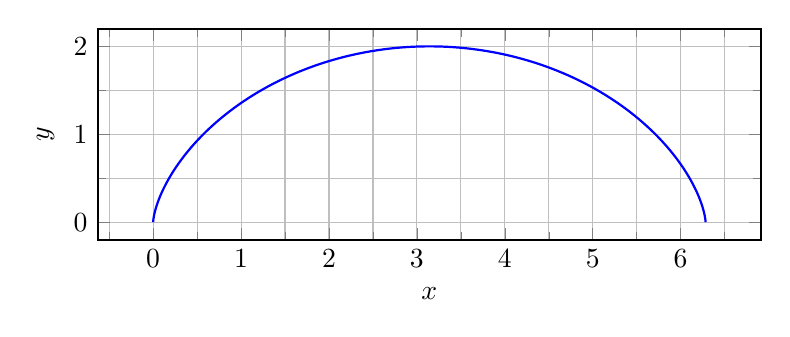
\begin{tikzpicture}
    \begin{axis}[
      axis equal image,
      width=10cm,
      height=5cm,
      xlabel={$x$},
      ylabel={$y$},
      domain=0:6.2832,
      samples=200,
      grid=both,
      minor tick num=1,
      thick
    ]
      % サイクロイド: a=1, φ∈[0,2π]
      \addplot [blue, thick] (
        {x - sin(deg(x))},
        {1 - cos(deg(x))}
      );
    \end{axis}
  \end{tikzpicture}
  \caption{サイクロイド曲線 $x = a(\varphi - \sin\varphi),\ y = a(1-\cos\varphi)$($a=1$,$\varphi\in[0,2\pi]$)}
\end{figure}

\end{document}
